%!TEX root = main.tex

\section{Decision procedure for $\strline_{\sf reg}$} \label{sec:decision}

In this section, we shall prove Theorem~\ref{thm-main}, i.e., the decidability of the path feasibility of $\strline_{\sf reg}$. 
%is decidable in XXX. \zhilin{complexity should be added}
%
We first show that semantically equivalent PSSTs can be effectively constructed from the $\extract$ and $\replaceall$ functions. 

\begin{lemma}\label{lem-extract}
A PSST $\cT_{\extract_{i,e}}$ can be constructed for $\extract_{i,e}(x)$ such that $\cR_{\cT_{\extract_{i,e}}} = \{(w, w') \mid w'= \extract_{i,e}(w)\}$.
\end{lemma}

\begin{lemma}\label{lem-replace}
A PSST $\cT_{\replaceall_{\pat, \rep}}$ can be constructed for $\replaceall_{\pat, \rep}(x)$ such that $\cR_{\cT_{\replaceall_{\pat, \rep}}} = \{(w, w') \mid w'= \replaceall_{\pat, \rep}(w)\}$.
\end{lemma}

With Lemma~\ref{lem-extract}-\ref{lem-replace}, the path feasibility of $\strline_{\sf reg}$ is reduced to the path feasibility of string-manipulating programs consisting of  a sequence of the statements of the form $z:=x \concat y$, $y:=\cT(x)$ and $\ASSERT{x \in \cA}$, where $\cT$ is a PSST and $\cA$ is an FA.  The class of programs is denoted by $\strline'_{\sf reg}$. We will  follow %the %backward computation %reasoning approach of 
the general OSTRICH framework \cite{CCH+18,CHL+19} to solve the path feasibility of $\strline'_{\sf reg}$, where the key is to show that the pre-images of regular languages  under PSSTs  are regular and can be computed effectively.

\begin{definition}[Pre-image]
For a string relation $R \subseteq \Sigma^* \times \Sigma^*$ and $L \subseteq \Sigma^*$, we define the \emph{pre-image} of $L$ under $R$ as $R^{-1}(L):=\{w \in \Sigma^* \mid \exists w'.\ w' \in L \mbox{ and } (w, w') \in R\}$. 
\end{definition}
 
\begin{lemma}[Pre-image of \PSST{}]
  \label{lem:psst_preimage}
  Given a \PSST{} $\psst = (Q_T, \Sigma$, $X$, $\delta_T$, $\tau_T$, $E_T$,  $q_{0, T}$, $F_T$) and an \FA{} $\Aut
  = (Q_A, \Sigma, \delta_A, q_{0, A}, F_A)$, we can compute an \FA{} $\cB = (Q_B,
  \Sigma, \delta_B, q_{0, B}, F_B)$ in exponential time  such that $\Lang(\cB) = \cR^{-1}_{\cT}(\Lang(\Aut))$.
\end{lemma}

With Lemma~\ref{lem:psst_preimage}, we  solve the path feasibility of $\strline'_{\sf reg}$ by repeating the following procedure, until no more assignment statements are left. Let $S$ be the current $\strline'_{\sf reg}$ program.
\begin{itemize}
\item If the last assignment statement of $S$ is $y:=\cT(x)$, then let $\ASSERT{y \in \cA_1}$, $\cdots$, $\ASSERT{y \in \cA_n}$ be an enumeration of all the assertion statements for $y$ in $S$. Compute $\cR^{-1}_\cT(\Lang(\cA_1))$ as an FA $\cB_1$, $\cdots$, and $\cR^{-1}_\cT(\Lang(\cA_n))$ as $\cB_n$. Remove  the assignment  $y:=\cT(x)$ and add the assertion statements $\ASSERT{x \in \cB_1}$; $\cdots$; $\ASSERT{x \in \cB_n}$. 
%
\item If the last assignment statement of $S$ is $z:=x \concat y$, then let $\ASSERT{z \in \cA_1}$, $\cdots$, $\ASSERT{z \in \cA_n}$ be an enumeration of all the assertion statements for $z$ in $S$. Compute $\concat^{-1}(\Lang(\cA_1))$, the pre-image of $\concat$ under $\Lang(\cA_1)$, as a collection of FA pairs $(\cB_{1,j}, \cC_{1,j})_{j \in [m_1]}$, $\cdots$, and $\concat^{-1}(\Lang(\cA_n))$ as $(\cB_{n, j}, \cC_{n,j})_{j \in [m_n]}$ (c.f. \cite{CHL+19}). Remove the assignment $z:=x \concat y$, nondeterministically choose the indices $j_1 \in [m_1], \cdots, j_n \in [m_n]$, and add the assertion statements $\ASSERT{x \in \cB_{1,j_1}}; \ASSERT{y \in \cC_{1, j_1}}$; $\cdots$; $\ASSERT{x \in \cB_{n,j_n}}; \ASSERT{y \in \cC_{n, j_n}}$. 
\end{itemize}

\begin{remark}
The aforementioned procedure extends the approach of backward reasoning proposed in \cite{CCH+18,CHL+19}. While standard one-way and two-way transducers were considered in \cite{CCH+18,CHL+19}, we introduce PSST, a new transducer model that covers the $\extract_{i,e}$ and $\replaceall_{\sf pat, rep}$ functions, where priorities are used to model the greedy/non-greedy semantics of $*$/$*?$ and string variables are used to store the matches of capturing groups. 
\end{remark}

It remains to prove Lemma~\ref{lem-extract}-\ref{lem:psst_preimage}, which will be the focus of the next two subsections.
% in Section~\ref{sec-extract-replace-to-psst}-\ref{sec-pre-image}.



%%%%%%%%%%%%%%%%%%%%%%%%%%%%%%%%%%%%%%%%%%%%%%%
\subsection{From $\extract$ and $\replaceall$ to PSST}\label{sec-extract-replace-to-psst}

At first, we can adapt the pNFA construction in \cite{BDM14}, which in turn is a variant of the standard Thompson construction \cite{Thompson68}, and show the following result. 

\begin{proposition}\label{prop-rwre-to-pfa}
For each $\cgexp$ $e$, a PFA $\cA_e$ can be constructed in linear time such that 
\begin{itemize}
\item $\cA_e$ has a unique initial state without incoming transitions and a unique final state without outgoing transitions,
%
\item for subexpression $e'$ of $e$, $\cA_e$ contains an isomorphic copy of $\cA_{e'}$ (i.e. the PFA constructed for $e'$), denoted by ${\sf Sub}_{e'}[\cA_e]$. 
\end{itemize}
\end{proposition}
%Let us use ${\sf Sub}_{e'}[\cA_e]$ to denote the isomorphic copy of $\cA_{e'}$ in $\cA_e$, as mentioned in Proposition~\ref{prop-rwre-to-pfa}.

%
%\begin{theorem}\label{thm-main}
%The path feasibility of $\strline_{\sf reg}$ is decidable.
%\end{theorem}
%




%\subsection{From $\regexp[\sf CG]$ to PFA}
%\label{construction:pnfa}

%\begin{figure*}
%	\centering
%	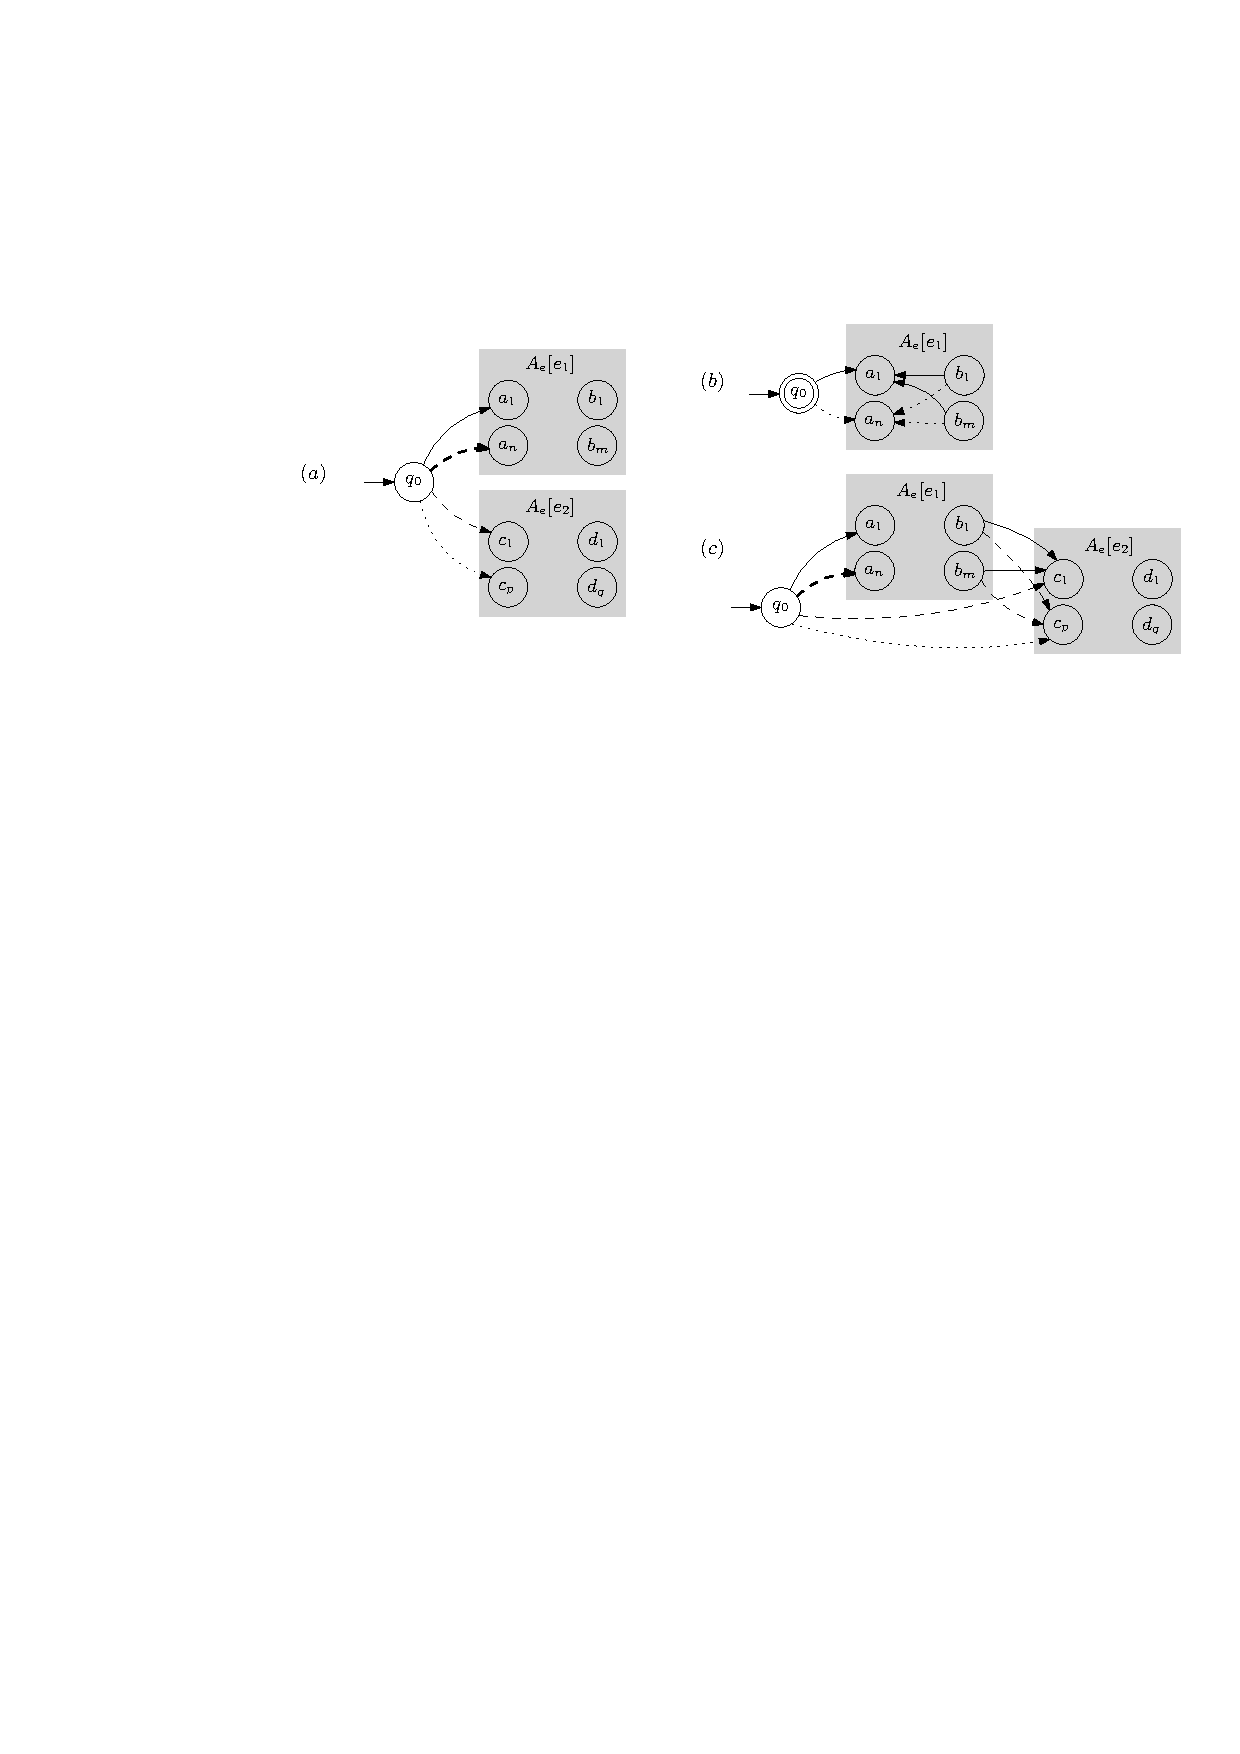
\includegraphics{pglushkov_01}
%	\caption{pNFA $A_e$ for (a) $e=e_1+e_2$ (b) $e=e_1^{\ast}$ and (c) $e=e_1 \concat e_2$ where $\varepsilon \in \Lang(e_1)$ and $\varepsilon \notin \Lang(e_2)$. A transition of lower priority is depicted thiner and more densely dotted. }
%	\label{fig:pglushkov}
%\end{figure*}

%For instance, if $e = (a (ab)^*)^*$ and $e' = a(ab)^*$, then $A_{e}[e']$ is the subgraph of $A_{e}$ comprising the states $\{a_1, a_2, b_3\}$ and the transitions $\{(a_1, a, a_2), (a_2, b, b_3), (b_3, a, a_2)\}$.
 
%Figure.\ref{fig:pglushkov} also illustrates the subgraphs corresponding to direct subexpressions of $e$.


%\begin{definition}
%Let $e \in \regexp[\sf CG]$ and $e'$ be a subexpression of $e$. Then a copy of $\cA_{e'}$ in $\cA_e = (Q, \Sigma, \delta, \tau, q_0, f_0)$ is a PFA $(Q', \Sigma, \delta', \tau', q'_0, f'_0)$ such that  
%\begin{itemize}
%\item $Q' \subseteq Q$, $q'_0, f'_0 \in Q'$, 
%\item $\delta'$ is the restriction of $\delta$ to $Q'$, with the outgoing transitions of $f'_0$ removed, specifically, for every $\sigma \in \Sigma$ and $q \in Q' \setminus \{f'_0\}$, $\delta'(q, \sigma) = \delta(q, \sigma)$, $\tau'(q) = \tau(q)$, $\delta'(f'_0, \sigma) = ()$, and $\tau'(f'_0) = ((); ())$,
%\item $(Q', \Sigma, \delta', \tau', q'_0, f'_0)$ is isomorphic to $\cA_{e'}$.
%\end{itemize}
%\end{definition}

%From the aforementioned recursive construction of $\cA_e$, we know that for each subexpression $e'$ of $e$, a PFA for $e'$, which is isomorphic to $\cA_{e'}$, is also constructed. Let us use ${\sf Sub}_{e'}[\cA_e]$ to denote this PFA for $e'$, which, roughly speaking, is a subgraph of $\cA_e$.


We are ready to prove Lemma~\ref{lem-extract} and Lemma~\ref{lem-replace}.
 
\begin{proof}[Lemma~\ref{lem-extract}]
%\paragraph*{Construction of $\cT_{\extract_{i,e}}$.} 
Let $e'$ be the subexpression corresponding to the $i$-th capturing group of $e$. In particular, if $i=0$, then $e' = e$. 

Suppose $\cA_e = (Q, \Sigma, \delta, \tau, q_0, f_0)$. Moreover, let $\cA^\dag_e = (Q^\dag, \Sigma, \delta^\dag, \tau^\dag, q^\dag_0, f^\dag_0)$ be an isomorphic copy of $\cA_e$, where every state $q$ in $\cA_e$ is replaced by $q^\dag$ in $\cA^\dag_e$. Let us use ${\sf Sub}_{e'}[\cA^\dag_e]$ to denote the isomorphic copy of ${\sf Sub}_{e'}[\cA_e]$ in $\cA^\dag_e$.

Intuitively, $\cT_{\extract_{i,e}}$ contains both $\cA_e$ and $\cA^\dag_e $, and its run comprises two stages: In the first stage, it simulates $\cA_e$. Later on, when it tries to enter a state in ${\sf Sub}_{e'}[\cA_e]$, it enters the second stage and goes to a state in ${\sf Sub}_{e'}[\cA^\dag_e]$, instead of ${\sf Sub}_{e'}[\cA_e]$, and stores the letters into $x$. It outputs $x$ in the state $f^\dag_0$.

Then $\cT_{\extract_{i,e}} = (Q  \cup Q^\dag \cup \{q'_0\}, \Sigma, X, \delta', \tau', E', q'_0, F')$ (see Figure~\ref{fig-psst-extract}), where 
\begin{itemize}
\item $q'_0 \not \in Q \cup Q^\dag$,
%
\item $X = \{x\}$,
%
%\item $\delta'$ is obtained from $\delta$ by adding $x: = x\sigma$ for each transition $(q, \sigma, q')$ in ${\sf Sub}_{e'}[\cA_e]$,  
%
\item $F'(f^\dag_0)= x$ and $F'(p)$ is undefined for all the other states in $p \in Q  \cup Q^\dag \cup \{q'_0\}$,
%
\item $\delta'$ and $\tau'$ are defined as follows,
\begin{itemize}
\item if $q_0$ does not occur in ${\sf Sub}_{e'}[\cA_e]$, then $\tau'(q'_0) = ((q_0), ())$, otherwise, $\tau'(q'_0) = ((q^\dag_0), ())$, 
%
\item for each $q \in Q$ such that $\delta(q) = (q_1, \cdots, q_n)$ and $q$ does not occur in ${\sf Sub}_{e'}[\cA_e]$, we have $\delta'(q) = (q'_1, \cdots, q'_n)$, where for each $i \in [n]$, if $q_i$ occurs in ${\sf Sub}_{e'}[\cA_e]$, then $q'_i = q^\dag_i$, otherwise, $q'_i = q_i$,
%
\item for each $q \in Q$ such that $\tau(q) = (P_1; P_2)$ and $q$ does not occur in ${\sf Sub}_{e'}[\cA_e]$, we have $\tau'(q) = (P'_1; P'_2)$, where $P'_1$ is obtained from $P_1$ by replacing each state $q \in P_1$ occurring in ${\sf Sub}_{e'}[\cA_e]$ with $q^\dag$, similarly for $P'_2$,
%
\item $\delta'$ (resp. $\tau'$) includes all the transitions in $\delta^\dag_e$ (resp. $\tau^\dag_e$),
%
\end{itemize}
%
\item for each transition $(q^\dag_1, \sigma, q^\dag_2)$ in ${\sf Sub}_{e'}[\cA^\dag_e]$ with $\sigma \in \Sigma$, we have $E'((q^\dag_1, \sigma, q^\dag_2))(x) = x \sigma$, and  on all the other transitions, $E'$ does not change the value of $x$.
%
\end{itemize}

\begin{figure}[ht]
\centering
%\rule{\linewidth}{0cm}
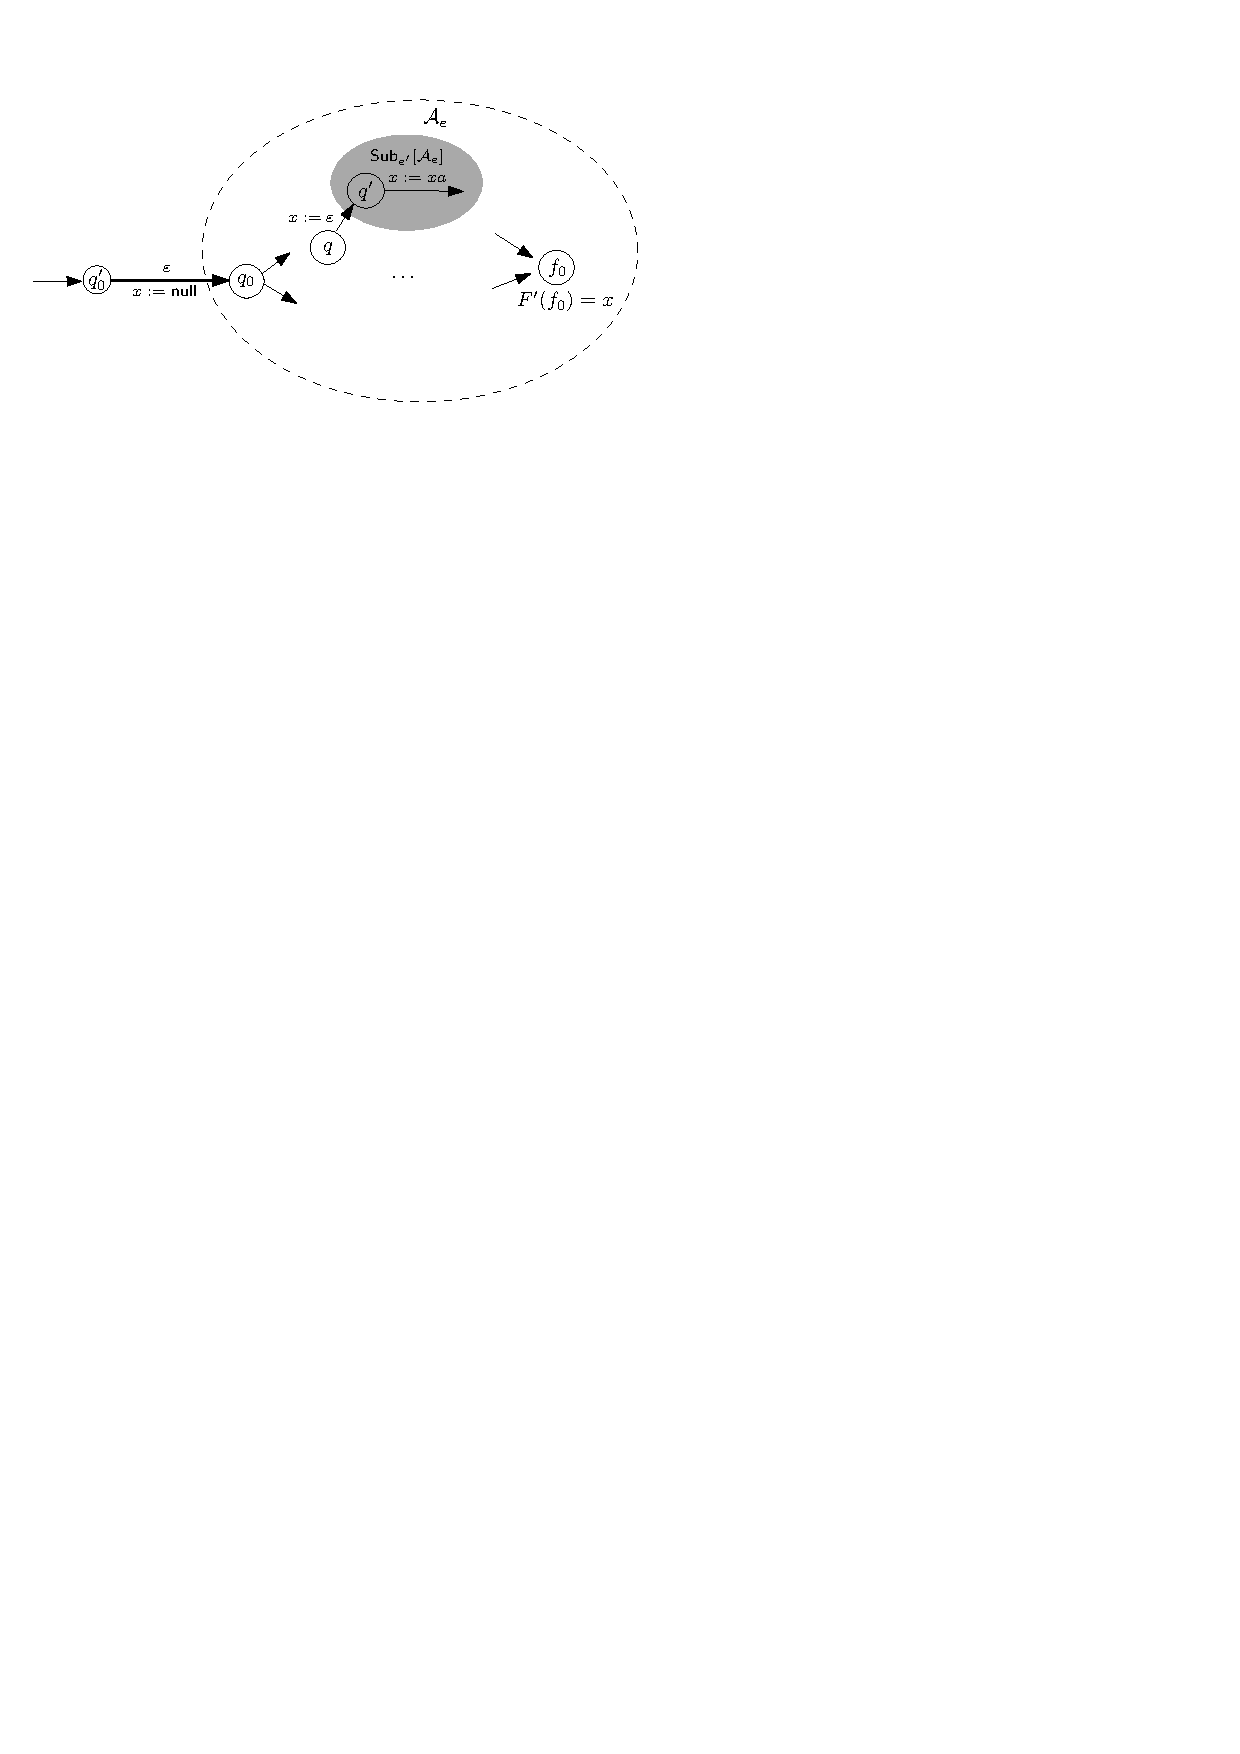
\includegraphics[width = \textwidth]{psst-extract.pdf}
\caption{The PSST for $\extract_{i,e}$}
\label{fig-psst-extract}
\end{figure}
\qed
\end{proof}


\begin{proof}[Lemma~\ref{lem-replace}]
%\paragraph*{Construction of $\cT_{\replaceall_{\pat, \rep}}$.} 
Let $\$i_1, \cdots, \$i_k$ with $i_1 < \cdots < i_k$ be an enumeration of all the references in $\rep$. 
Moreover, for every $j \in [k]$, let $e'_{i_j}$ be the subexpression of $\pat$ corresponding to the $i_j$-th capturing group.

Suppose $\cA_\pat = (Q, \Sigma, \delta, \tau, q_0, f_0)$. Then $\cT_{\replace_{\pat,\rep}}$ is obtained from $\cA_\pat$ by adding a fresh states $q'_0$ such that (see Figure~\ref{fig-psst-replace})
\begin{itemize}
\item $\cT_{\replace_{\pat,\rep}}$ goes from $q'_0$ to $q_0$ via an $\varepsilon$-transition of higher priority than the non-$\varepsilon$-transitions, in order to search the first match of $\pat$ starting from the current position, 
%
\item when $\cT_{\replace_{\pat,\rep}}$ stays at $q'_0$, it keeps appending the current letter to the end of $x_0$, 
%
\item starting from $q_0$, $\cT_{\replace_{\pat,\rep}}$ simulates $\cA_\pat$ and stores the matches of the $\$i_1$-th, $\ldots$, $\$i_k$-th capturing groups of $\pat$ into the string variables $x_1, \cdots, x_k$ respectively,   
%
\item when the first match of $\pat$ is found, $\cT_{\replace_{\pat,\rep}}$ goes from $f_0$ to $q'_0$ via an $\varepsilon$-transition, appends the replacement string, which is $\rep[x_1/\$_{i_1}, \cdots, x_k/\$_{i_k}]$, to the end of $x_0$, and keeps searching for the next match of $\pat$.
\end{itemize}

\begin{figure}[ht]
\centering
%\rule{\linewidth}{0cm}
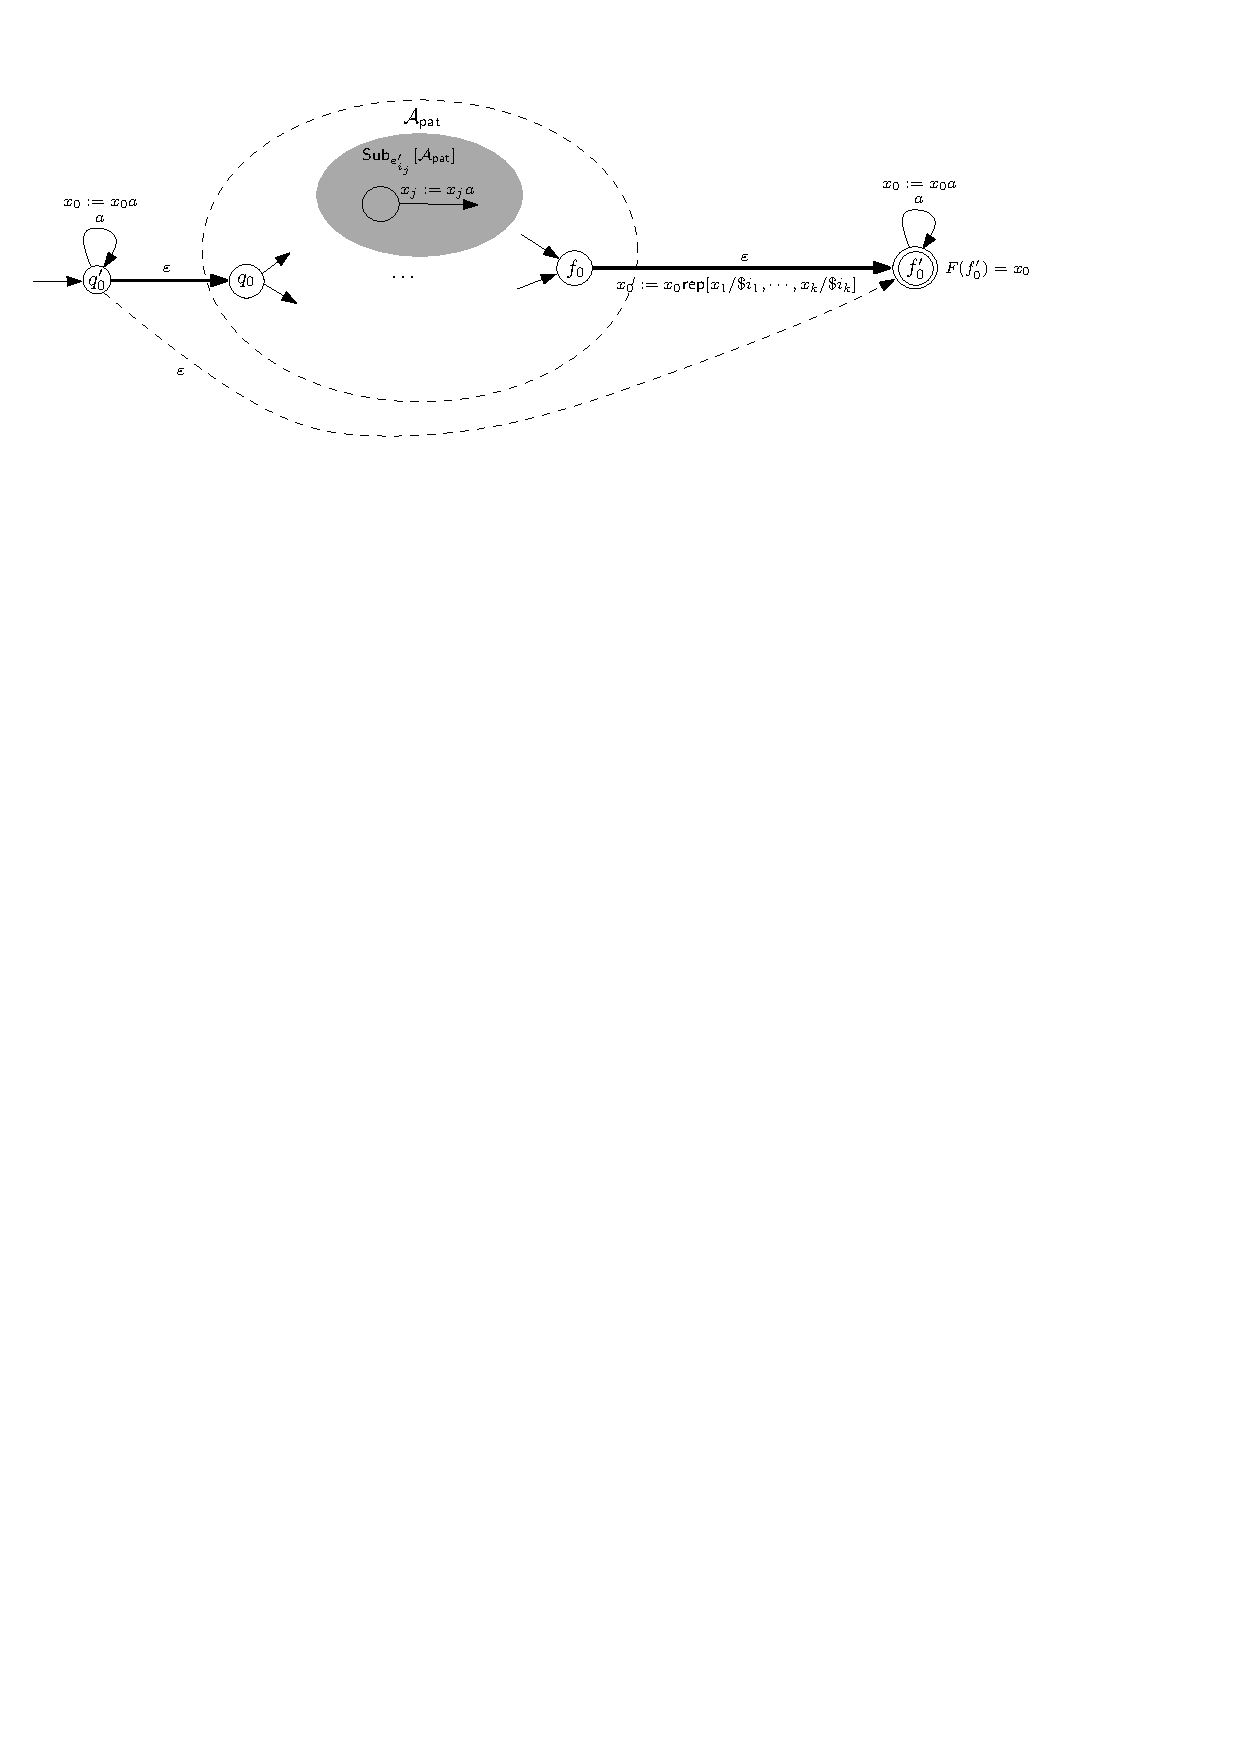
\includegraphics[scale=0.7]{psst-replace.pdf}
\caption{The PSST for $\replace_{\pat,\rep}$}
\label{fig-psst-replace}
\end{figure}

Formally, $\cT_{\replaceall_{\pat, \rep}} =$ $(Q \cup \{q'_0\}$, $\Sigma$, $X$, $\delta'$, $\tau', E, q'_0, F)$ where
\begin{itemize}
\item $q'_0 \not \in Q$,

\item  $X = \{x_0, x_1, \cdots, x_k\}$,
%
\item $F(q'_0) = x_0$, and $F(q')$ is undefined for every $q' \in Q$,
%
\item $\delta'$ and $\tau'$ are obtained from $\delta$ and $\tau$ as follows,
\begin{itemize}
\item $\delta'(q'_0, \sigma) = (q'_0)$ for every $\sigma \in \Sigma$, and $\tau'(q'_0) = ((q_0); ())$,
%
\item for every $q \in Q \setminus \{f_0\}$ and $\sigma \in \Sigma$, $\delta'(q, \sigma) = \delta(q, \sigma)$ and $\tau'(q) = \tau(q)$, 
%
\item $\delta'(f_0, \sigma) = ()$ for every $\sigma \in \Sigma$ and $\tau'(f_0) = ((q'_0); ())$,
\end{itemize}
%
\item $E$ is defined as follows, 
\begin{itemize}
\item for every transition $(q, \sigma, q')$ with $\sigma \in \Sigma^\varepsilon$ in $\cA_\pat$, $E(q, \sigma, q')(x_0) = x_0$,
%
\item for every transition $(q, \sigma, q')$ with $\sigma \in \Sigma^\varepsilon$ and $j \in [k]$,  if $(q, \sigma, q')$ occurs in ${\sf Sub}_{e'_{i_j}}[\cA_\pat]$, then $E(q, \sigma, q')(x_j) = x_j\sigma$, otherwise, $E(q, \sigma, q')(x_j) = x_j$,
%
%\item for all the other transitions $(q, \sigma, q')$ with $\sigma \in \Sigma^\varepsilon$ in $\cA_e$, we have $E(q, \sigma, q')(x) = x$, 
%
\item  for every $\sigma \in \Sigma$ and $j \in [k]$, $E(q'_0, \sigma, q'_0)(x_0) = x_0\sigma$ and $E(q'_0, \sigma, q'_0)$$(x_j) = x_j$, 

\item $E(q'_0, \varepsilon, q_0)(x_j) = x_j$ for every $j \in [k] \cup \{0\}$, 
%
\item $E(f_0, \varepsilon, q'_0)(x_0) = x_0 \rep[x_1/\$i_1,\ldots, x_k/\$i_k]$, and for every $j \in [k]$, we have $E(f_0, \varepsilon, q'_0)(x_j) = \varepsilon$.

\end{itemize}
%
\end{itemize}
\qed
\end{proof}


\subsection{Computing the pre-image of \PSST}\label{sec-pre-image}

In this subsection, we are going to show Lemma~\ref{lem:psst_preimage}, namely, how to compute pre-images of regular languages under PSSTs.

%\tl{another way is to first define B as a PFA, could make the construction a bit modular?}\zhilin{Add a counter example for this natural idea.}
 
Let $\psst = (Q_T, \Sigma$, $X, \delta_T, \tau_T, E_T,  q_{0, T}, F_T)$ be a \PSST{}  and $\Aut
  = (Q_A, \Sigma$, $\delta_A$, $q_{0, A}$, $F_A)$ be an \FA{}. Without loss of generality, we assume that $\Aut$ contains no $\varepsilon$-transitions. 

To illustrate the intuition of the FA construction, let us start with the following natural idea of firstly constructing a PFA $\cB$ for the pre-image: $\cB$ simulates a run of $\psst$ on $w$, and, for each $x \in X$, records an $\Aut$-abstraction of the string stored in $x$, that is, the set of state pairs $(p, q) \in Q_A \times Q_A$ such that starting from $p$, $\Aut$ can reach $q$ after reading the string stored in $x$. Specifically, the states of $\cB$ are of the form $(q, \rho)$ with $q \in Q$ and $\rho \in (\cP(Q_A \times Q_A ))^{X}$. Moreover, the priorities of $\cB$ inherit those of $\Aut$. The PFA $\cB$ is then transformed to an equivalent FA by simply dropping all priorities. We refer to this FA as $\cB'$.

Nevertheless, it turns out that this construction method is flawed: A string $w$ is in $\cR^{-1}_{\cT}(\Lang(\Aut))$ iff the (unique) accepting run of $\cT$ on $w$ produces an output $w'$ that is accepted by $\Aut$. However, a string $w$ is accepted by $\cB'$ iff \emph{there is a run of $\cT$ on $w$, not necessarily of the highest priority}, producing an output $w'$ that is accepted by $\Aut$. The following example illustrates the flaw of the construction above.

\begin{example}
\label{pre-image-count-examp}
Let $\cT_{\tt match_{decimalReg,1}}$ be the PSST in Figure~\ref{fig-psst-exmp} and $\cA$ be the FA corresponding to the regular expression $\{1,\cdots,9\}^*$, specifically, $\cA= (\{p_0\}$, $\{0,\cdots,9\}$, $\delta_A$, $p_0, \{p_0\})$, where $\delta_A = \{(q_0, \ell, q_0) \mid \ell = 1, \cdots, 9\}$.
%  in Figure~\ref{fig-pre-image-count-exmp}, that is, 
%\begin{itemize}
%\item $\cT=(\{q_0, q_1, q_2\}, \{a,b,c\}, \{x_0\}, \delta_T, \tau_T, E_T, q_0, F_T)$, where $\delta_T(q_0, \sigma) = (q_0)$, $\delta_T(q_1, a) = (q_1)$, $\delta_T(q_2, \sigma) = (q_2)$, $\tau_T(q_0) = ((q_1); ())$, $\tau_T(q_1)=((q_0, q_2);())$, and $\tau_T(q_2)= ((); ())$, $E_T(q_0, \sigma, q_0) (x_0) = x_0 \sigma$, $E_T(q_1, \varepsilon, q_0) (x_0) = x_0 c$, $E_T(q_1, \varepsilon, q_2) (x_0) = x_0 c$, $E_T(q_2, \sigma, q_2) (x_0) = x_0 \sigma$, for $\sigma \in\{ a, b\}$. Moreover, $F_T(q_2)= x_0$;
%
%\item $\cA = (\{p_0\}, \{a,b,c\}, \delta_A, p_0, \{p_0\})$, where $\delta_A$ = $\{(p_0, \sigma, p_0)$ $\mid \sigma = b, c\}$.
%\end{itemize}

Let us consider $w = 10$. The accepting run of $\cT_{\tt match_{decimalReg,1}}$ on $w$ is $q_0 \xrightarrow[x_1:=x_11]{1} q_1 \xrightarrow[x_1:=x_10]{0} q_1 \xrightarrow{\varepsilon} q_2 \xrightarrow{\varepsilon} q_3 \xrightarrow{\varepsilon} q_4 \xrightarrow{\varepsilon} q_5 \xrightarrow{\varepsilon} q_6$, producing an output $10 \not \in \Lang(\cA)$. Therefore, $10 \not \in \cR_\cT^{-1}(\Lang(\cA))$. Nevertheless, if we consider the FA $\cB'$ constructed from $\cT$ and $\cA$,  it turns out that $\cB'$ does accept $w$, witnessed by the run $(q_0, \{(p_0,p_0)\}) \xrightarrow{1} (q_1, \{(p_0, p_0)\}) \xrightarrow{\varepsilon} (q_2, \{(p_0, p_0)\}) \xrightarrow{\varepsilon}  (q_3, \{(p_0, p_0)\}) \xrightarrow{\varepsilon}  (q_4, \{(p_0, p_0)\}) \xrightarrow{\varepsilon}  (q_5, \{(p_0, p_0)\}) \xrightarrow{0}  (q_5, \{(p_0, p_0)\}) \xrightarrow{\varepsilon}  (q_6, \{(p_0, p_0)\})$. On the other hand, the run of $\cB'$ corresponding to the accepting run of $\cT$ on $w$, i.e. $(q_0, \{(p_0, p_0)\}) \xrightarrow{1} (q_1, \{(p_0, p_0)\}) \xrightarrow{0} (q_1, \emptyset) \xrightarrow{\varepsilon}  (q_2, \emptyset) \xrightarrow{\varepsilon} (q_3, \emptyset) \xrightarrow{\varepsilon} (q_4, \emptyset) \xrightarrow{\varepsilon} (q_5, \emptyset) \xrightarrow{\varepsilon} (q_6, \emptyset)$, is not accepting, where $\{(p_0,p_0)\}$ and $\emptyset$ are the $\cA$-abstractions of $x_1$.
\end{example}

%%%%%%%%%%%%%%%%%%%%%%%%%%%%%%
%%%%%%%%%%%%%%%%%%%%%%%%%%%%%%
\hide{
\begin{example}
\label{pre-image-count-examp}
Let $\cT$ be the PSST and $\cA$ be the FA in Figure~\ref{fig-pre-image-count-exmp}, that is, 
\begin{itemize}
\item $\cT=(\{q_0, q_1, q_2\}, \{a,b,c\}, \{x_0\}, \delta_T, \tau_T, E_T, q_0, F_T)$, where $\delta_T(q_0, \sigma) = (q_0)$, $\delta_T(q_1, a) = (q_1)$, $\delta_T(q_2, \sigma) = (q_2)$, $\tau_T(q_0) = ((q_1); ())$, $\tau_T(q_1)=((q_0, q_2);())$, and $\tau_T(q_2)= ((); ())$, $E_T(q_0, \sigma, q_0) (x_0) = x_0 \sigma$, $E_T(q_1, \varepsilon, q_0) (x_0) = x_0 c$, $E_T(q_1, \varepsilon, q_2) (x_0) = x_0 c$, $E_T(q_2, \sigma, q_2) (x_0) = x_0 \sigma$, for $\sigma \in\{ a, b\}$. Moreover, $F_T(q_2)= x_0$;
%
\item $\cA = (\{p_0\}, \{a,b,c\}, \delta_A, p_0, \{p_0\})$, where $\delta_A$ = $\{(p_0, \sigma, p_0)$ $\mid \sigma = b, c\}$.
\end{itemize}

Let us consider $w = a$. The accepting run of $\cT$ on $w$ is $q_0 \xrightarrow{\varepsilon} q_1 \xrightarrow[x_0:=x_0c]{\varepsilon} q_0 \xrightarrow[x_0:=x_0a]{a} q_0 \xrightarrow{\varepsilon} q_1 \xrightarrow[x_0:=x_0c]{\varepsilon} q_2$, producing an output $cac \not \in \Lang(\cA)$. Therefore, $a \not \in \cR_\cT^{-1}(\Lang(\cA))$. Nevertheless, if we consider the FA $\cB'$ constructed from $\cT$ and $\cA$,  it turns out that $\cB'$ does accept $w$, witnessed by the run $(q_0, \{(p_0,p_0)\}) \xrightarrow{\varepsilon} (q_1, \{(p_0,p_0)\}) \xrightarrow{a} (q_1, \{(p_0, p_0)\}) \xrightarrow{\varepsilon}  (q_2, \{(p_0, p_0)\})$. On the other hand, the run of $\cB'$ corresponding to the accepting run of $\cT$ on $w$, i.e. $(q_0, \{(p_0,p_0)\}) \xrightarrow{\varepsilon} (q_1, \{(p_0,p_0)\}) \xrightarrow{\varepsilon} (q_0, \{(p_0, p_0)\}) \xrightarrow{a}  (q_0, \emptyset) \xrightarrow{\varepsilon} (q_1, \emptyset) \xrightarrow{\varepsilon} (q_2, \emptyset)$, is not accepting, where $\{(p_0,p_0)\}$ and $\emptyset$ are the $\cA$-abstractions of $x_0$.
\end{example}

\begin{figure}[ht]
\centering
%\rule{\linewidth}{0cm}
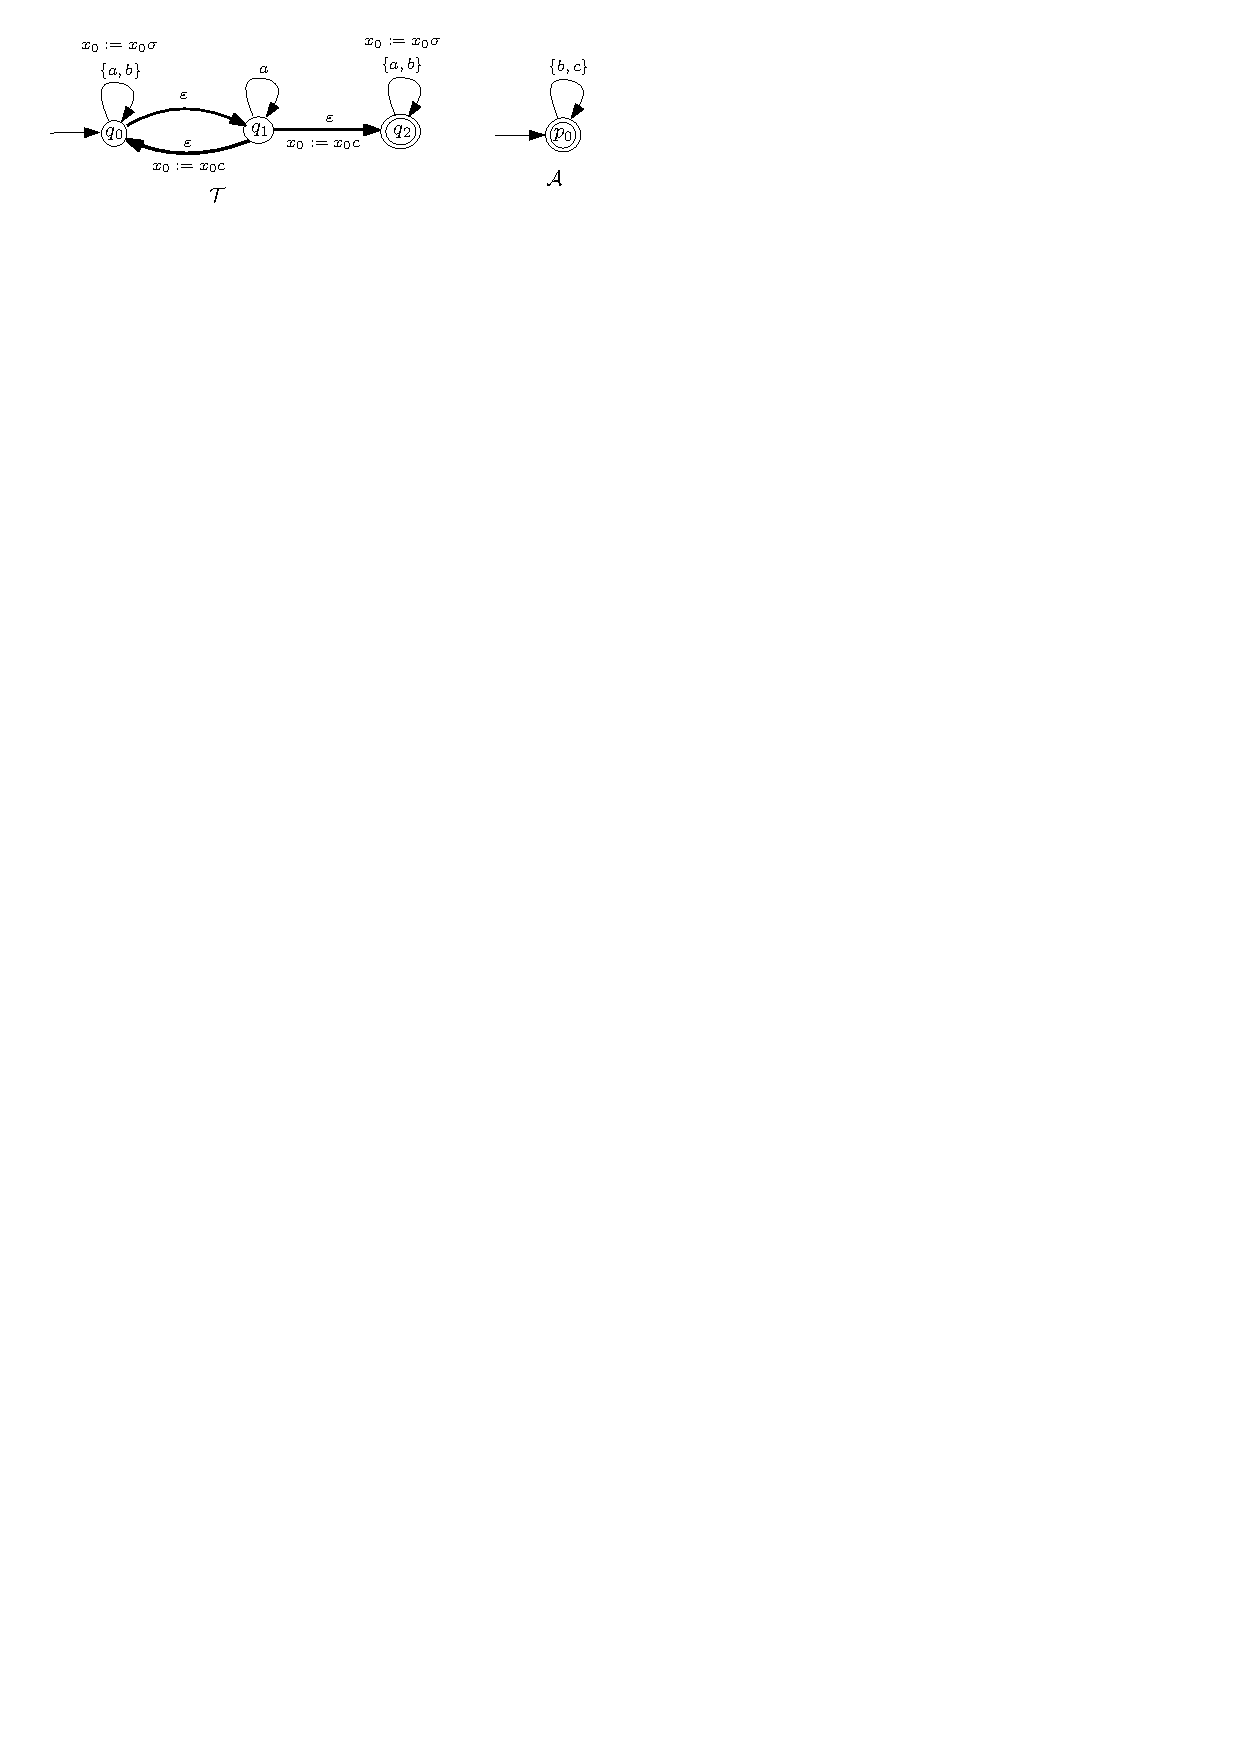
\includegraphics[scale=0.8]{pre-image-counter-example.pdf}
\caption{A counterexample to disprove the flawed pre-image construction method}
\label{fig-pre-image-count-exmp}
\end{figure}
}
%%%%%%%%%%%%%%%%%%%%%%%%%%%%%%%%
%%%%%%%%%%%%%%%%%%%%%%%%%%%%%%%%

\begin{proof}[Lemma~\ref{lem:psst_preimage}]
Let $\psst = (Q_T, \Sigma$, $X, \delta_T, \tau_T, E_T,  q_{0, T}, F_T)$ be a \PSST{} and $\Aut
  = (Q_A, \Sigma, \delta_A, q_{0, A}, F_A)$ be an \FA{}. For convenience, we use $\cE(\tau_T)$ to denote $\{(q, q') \mid q' \in \tau_T(q)\}$.

Our goal is to construct a FA $\cB$ that simulates the run of $\psst$ on $w$, and, for each $x \in X$, records an $\Aut$-abstraction of the string stored in $x$, that is, the set of state pairs $(p, q) \in Q_A \times Q_A$ such that starting from $p$, $\Aut$ can reach $q$ after reading the string stored in $x$. To simulate the runs of $\psst$, it is necessary to record all the states accessible from a run of higher priority to ensure the current run is an accepting run of $\psst$ of highest priority. Moreover, $\cB$ also remembers the set of $\varepsilon$-transitions of $\cT$ after the latest non-$\varepsilon$-transition to ensure that no transition occurs twice in a sequence of $\varepsilon$-transitions of $\cT$.

Specifically, each state of $\cB$ is of the form $(q, \rho, \Lambda, S)$, where $q \in Q_T$, $\rho \in (\cP(Q_A \times Q_A ))^{X}$, $\Lambda \subseteq \cE(\tau_T)$, and $S \subseteq Q_T$. 
For a state $(q, \rho, \Lambda, S)$, our intention for $S$ is that the states in it are those that can be reached in the runs of higher priorities than the current run, by reading the same sequence of letters and applying the $\varepsilon$-transitions as many as possible. Note that when recording in $S$ all the states accessible from a run of higher priority, we do not take the non-repetition of $\varepsilon$-transitions into consideration since if a state is reachable by a sequence of $\varepsilon$-transitions where some $\varepsilon$-transitions are repeated, then there exists also a sequence of non-repeated $\varepsilon$-transitions reaching the state. 
Moreover, when simulating a $\sigma$-transition of $\cT$ (where $\sigma \in \Sigma$) at a state $(q, \rho, \Lambda, S)$, suppose $\delta_T(q, \sigma) = (q_1, \cdots, q_m)$ and $\tau_T(q) = (P_1, P_2)$, then $\cB$ nondeterministically chooses $q_i$ and goes to the state $(q_i, \rho', \emptyset, S')$, where 
\begin{itemize}
\item $\rho'$ is obtained from $\rho$ and $E_T(q, \sigma, q_i)$, 
%
\item $\Lambda$ is reset to $\emptyset$,
% 
\item all the states obtained from $S$ by applying  a $\sigma$ transition should be \emph{saturated by $\varepsilon$-transitions} and put into $S'$, more precisely, all the states reachable from $S$ by first applying a $\sigma$-transition, then a sequence of $\varepsilon$-transitions, should be put into $S'$,
%
\item moreover, all the states obtained from $q_1,\cdots, q_{i-1}$ (which are of higher priorities than $q_i$) by saturating with $\varepsilon$-transitions should be put into $S'$,
%
\item finally, all the states obtained from those in $P'_1 = \{q' \in P_1 \mid (q, q') \not \in \Lambda\}$ (which are of higher priorities than $q_i$) by saturating with non-$\Lambda$ $\varepsilon$-transitions first (i.e. the $\varepsilon$-transitions that do not belong to $\Lambda$), and applying a $\sigma$ transition next, finally saturating with $\varepsilon$-transitions again, should be put into $S'$, (note that according to the semantics of PSST, the $\varepsilon$-transitions in $\Lambda$ should be avoided when defining $P'_1$ and saturating the states in $P'_1$ with $\varepsilon$-transitions). 
\end{itemize}
%For technical reasons, when constructing $\cB$, we assume that this saturation happens when a state is added to $S$ for the first time. Therefore, at a state $(q, \rho, \Lambda, S)$, all the states reachable from the states in $S$ by sequences of $\varepsilon$-transitions in $\cT$ have already been in $S$.

Before the formal construction of $\cB$, we introduce some notations.
\begin{itemize}
\item For $S \subseteq Q_T$, $\delta^{(ip)}_T(S, a) = \{q'_1 \mid \exists q_1 \in S, q'_1 \in \delta_T(q_1, a)\}$.
%
\item For $q \in Q_T$,  if $\tau_T(q) = (P_1, P_2)$, then $\tau^{(ip)}_T(\{q\})=S$ such that $S = P_1 \cup P_2$. 
Moreover, for $S \subseteq Q_T$, we define $\tau^{(ip)}_T(S) = \bigcup \limits_{q \in S} \tau^{(ip)}_T(\{q\})$. We also use $\big(\tau^{(ip)}_T\big)^\ast$ to denote the $\varepsilon$-closure of $\cT$, namely, $\big(\tau^{(ip)}_T\big)^\ast(S) = \bigcup \limits_{n \in \Nat} \big(\tau^{(ip)}_T\big)^{n}(S)$, where $\big(\tau^{(ip)}_T\big)^{0}(S) = S$, and for $n \in \Nat$, $\big(\tau^{(ip)}_T\big)^{n+1}(S) = \tau^{(ip)}_T\big(\big(\tau^{(ip)}_T\big)^{n}(S)\big)$. 
%
\item For $S \subseteq Q_T$ and $\Lambda \subseteq  \cE(\tau_T)$, we use $\big(\tau^{(ip)}_T \backslash \Lambda\big)^\ast(S)$ to denote the set of states reachable from $S$ by sequences of $\varepsilon$-transitions where {\it no} transitions $(q, \varepsilon, q')$ such that $(q, q') \in \Lambda$ are used.
%
%We also use $(\tau^{(ip)}_T)^\ast$ to denote the reflexive transitive closure of $\tau^{(ip)}_T$. \tl{here $(\tau^{(ip)}_T)$ is defined as a function... you mean function composition?}
%\zhilei{I think we can just use the term 'epsilon closure' here?}
%\item For $\sigma \in \Sigma$ and $S \subseteq Q_T$,  we use $\tau^+_T[a, S]$ to denote the set of states that can be obtained from 
% 
\item For $\rho \in (\cP(Q_A \times Q_A ))^{X}$ and $s \in X \rightarrow (X \cup \Sigma)^{\ast}$, we use $s(\rho)$ to denote $\rho'$ that is obtained from $\rho$ as follows: For each $x \in X$, if $s(x) = \varepsilon$, then $\rho'(x) = \{(p, p) \mid p \in Q_A\}$, otherwise, let $s(x) = b_1 \cdots b_\ell$ with $b_i \in \Sigma \cup X$ for each $i \in [\ell]$, then $\rho'(x) = \theta_1 \circ \cdots \circ \theta_\ell$, where $\theta_i = \delta^{(b_i)}_A$ if $b_i \in \Sigma$, and $\theta_i = \rho(b_i)$ otherwise.
\end{itemize}

We are ready to present the formal construction of $\cB =  (Q_B$, $\Sigma$, $\delta_B$, $q_{0, B}, F_B)$. 
\begin{itemize}
\item $Q_B = Q_T \times (\cP(Q_A \times Q_A ))^{X} \times \cP(\cE(\tau_T)) \times \cP(Q_T)$, 
%(Intuitively, the letter $\sigma$ in $(q, \sigma, \rho, S) \in Q_B$ means the next letter to be read at $q$, with $\bot$ represents the end of the input.)

\item $q_{0, B} = (q_{0,T}, \rho_{\varepsilon}, \emptyset, \emptyset)$ where $\rho_{\varepsilon} (x) = \{(q, q) \mid q \in Q\}$ for each $x \in X$,

\item $\delta_{B}$ comprises 
\begin{itemize}
%\item the tuples $(q'_0, \varepsilon, ((q_{0,T},\sigma), \rho_{\varepsilon}, \emptyset))$ where $\sigma \in \Sigma$, $\rho_{\varepsilon} (x) = \{(q, q) \mid q \in Q\}$ for each $x \in X$, 
%
\item the tuples $((q, \rho, \Lambda, S), \sigma, (q_i, \rho', \Lambda', S'))$ such that  
%there exists $s \in \left((X \cup \Sigma\right)^*)^X)$ satisfying
\begin{itemize}
\item $\sigma \in \Sigma$, 
%$\sigma' \in \Sigma \cup \{\bot\}$, 
%
\item $\delta_T (q, \sigma) = (q_1, \ldots, q_i, \ldots, q_m)$, 
%
\item $s = E(q, \sigma, q_i)$, 
%
\item $\rho' = s(\rho)$,
%
\item $\Lambda' = \emptyset$, (Intuitively, $\Lambda$ is reset.)
%
\item let $\tau_T(q) = (P_1, P_2)$, then $S' = \big(\tau^{(ip)}_T\big)^\ast\big(\{ q_1$, $\ldots$, $q_{i - 1} \} \cup \delta^{(ip)}_T\big(S \cup \big(\tau^{(ip)}_T \setminus \Lambda\big)^\ast(P'_1), \sigma\big)\big)$, where $P'_1 = \{q' \in P_1 \mid (q, q') \not \in \Lambda\}$;  
%(Note that according to the semantics of PSSTs, when computing the set of states reachable from $q$ through an $\varepsilon$-transition to some $q' \in P_1$ first and a sequence of $\varepsilon$-transitions starting from $q'$ next, the transitions $(q'', \varepsilon, q''')$ with $(q'', q''') \in \Lambda$ should be excluded. )
%
\end{itemize}
%
\item the tuples $((q, \rho, \Lambda, S), \varepsilon, (q_i, \rho', \Lambda', S'))$ such that 
%there exists $s \in \left((X \cup \Sigma\right)^*)^X$ satisfying
\begin{itemize}
%, $\sigma' \in \Sigma \cup \{\bot\}$, 
%
\item $\tau_T(q) = ((q_1, \ldots, q_i, \ldots, q_m); \cdots)$, 
%
\item $(q, q_i) \not \in \Lambda$,

\item $s = E(q, \varepsilon, q_i)$, 
%
\item $\rho' = s(\rho)$,
%
\item $\Lambda' = \Lambda \cup \{(q, q_i)\}$, 
%
\item $S' =  S \cup \big(\tau^{(ip)}_T \backslash \Lambda \big)^\ast(\{ q_j \mid j \in [i-1], (q, q_j) \not \in \Lambda \})$;
%
%$\rho'(x) = \theta_\ell$ such that $\theta_0 = \{(p,p) \mid p \in Q_A\}$, and for each $i \in [\ell]$, if $b_i \in \Sigma$, then $\theta_i = \{(p, p') \mid (p, p'') \in \theta_{i-1}, (p'', b_i, p') \in \delta_A \mbox{ for some } p''\}$, otherwise, $\theta_i = \theta_{i-1} \cdot \rho(x)$. 
\end{itemize}
%

\item the tuples $((q, \rho, \Lambda, S), \varepsilon, (q_i, \rho', \Lambda', S'))$ such that 
%there exists $s \in \left((X \cup \Sigma\right)^*)^X$ satisfying
\begin{itemize}
%\item $\sigma \in \Sigma$, 
%$\sigma' \in \Sigma \cup \{\bot\}$, 
%
\item $\tau_T (q) = ((q'_1, \ldots, q'_n); (q_1, \ldots, q_i, \ldots, q_m))$, 
%
\item $(q, q_i) \not \in \Lambda$,
%
\item $s = E(q, \varepsilon, q_i)$,
%
\item $\rho' = s(\rho)$,
%
\item $\Lambda' = \Lambda \cup \{(q, q_i)\}$, 
%
\item $S' = S \cup \{q\} \cup \big(\tau^{(ip)}_T \backslash \Lambda \big)^\ast\big(\big\{q'_j \mid j \in [n], (q, q'_j) \not \in \Lambda \big\} \cup \big\{q_j \mid j \in [i-1], (q, q_j) \not \in \Lambda \big\} \big)$. (Note that here we include $q$ into $S'$, since the non-$\varepsilon$-transitions out of $q$ have higher priorities than the transition $(q, \varepsilon, q_i)$.)
%
%$\rho'(x) = \theta_\ell$ such that $\theta_0 = \{(p,p) \mid p \in Q_A\}$, and for each $i \in [\ell]$, if $b_i \in \Sigma$, then $\theta_i = \{(p, p') \mid (p, p'') \in \theta_{i-1}, (p'', b_i, p') \in \delta_A \mbox{ for some } p''\}$, otherwise, $\theta_i = \theta_{i-1} \cdot \rho(x)$. 
\end{itemize}
\end{itemize}
\item
Moreover, $F_B$ is the set of states $(q, \rho, \Lambda, S) \in Q_B$ such that
\begin{enumerate}
  \item $F_T (q)$ is defined,
%
  \item for any $q' \in S$, $F_T (q')$ is not defined,
  %
  \item if $F_T(q) = \varepsilon$, then $q_{0, A}  \in F_A$, otherwise, 
let $F_T(q) = b_1 \cdots b_\ell$ with $b_i \in \Sigma \cup X$ for each $i \in [\ell]$, then $(\theta_1 \circ \cdots \circ \theta_\ell) \cap (\{q_{0,A}\} \times F_A) \neq \emptyset$, where for each $i \in [\ell]$, if $b_i \in \Sigma$, then $\theta_i = \delta^{(b_i)}_A$, otherwise, $\theta_i = \rho(b_i)$.
\end{enumerate}
\end{itemize}
\end{proof}

Note that the above construction  does not utilize the so-called \tmtextit{copyless} property \cite{AC10,AD11},
  thus it works for general, or \textit{copyful} \PSST{} \cite{FR17}.

\begin{example}
Let us continue Example~\ref{pre-image-count-examp}. Suppose $\cT_{\tt match_{decimalReg,1}} = (Q_T, \Sigma$, $X, \delta_T$, $\tau_T, E_T,  q_{0, T}, F_T)$. Then the FA defining $\cR^{-1}_{\cT_{\tt match_{decimalReg,1}}}(\Lang(\Aut))$ constructed by using the aforementioned procedure is illustrated in Figure \ref{fig-psst-preimage-exmp}, where the final states are those boxed states, moreover, the states reachable from $(q_2, \emptyset, \{(q_1,q_2)\}, \{q_1\})$ are omitted because no final states are unreachable from those states, which are therefore redundant. Let us exemplify the construction by considering the state $(q_5, \{(p_0,p_0)\}, \{(q_1,q_2), (q_2,q_3), (q_3,q_4), (q_4, q_5)\}, \{q_1,q_3\})$. For each letter $\ell \in \{0,\cdots, 9\}$, the state $(q_5, \{(p_0,p_0)\}, \emptyset, \{q_1,q_2, q_3, q_4, q_5, q_6\})$ is reached from it, since $\delta(q_1,\ell) = (q_1)$ and $(\tau^{(ip)}_T)^*(\{q_1\}) = \{q_1, q_2, q_3, q_4, q_5, q_6\}$. Note that the state $(q_6, \{(p_0,p_0)\}, \{(q_5,q_6)\}, \{q_1, q_2, q_3, q_4, q_5, q_6\})$ is not a final state since $q_6$ belongs to the last component of the state and $F_T(q_6)$ is defined.
%For efficiency, we minimize the FA after the construction. See Section \ref{sect:impl} for implementation details.
\end{example}


\begin{figure}[ht]
\centering
%\rule{\linewidth}{0cm}
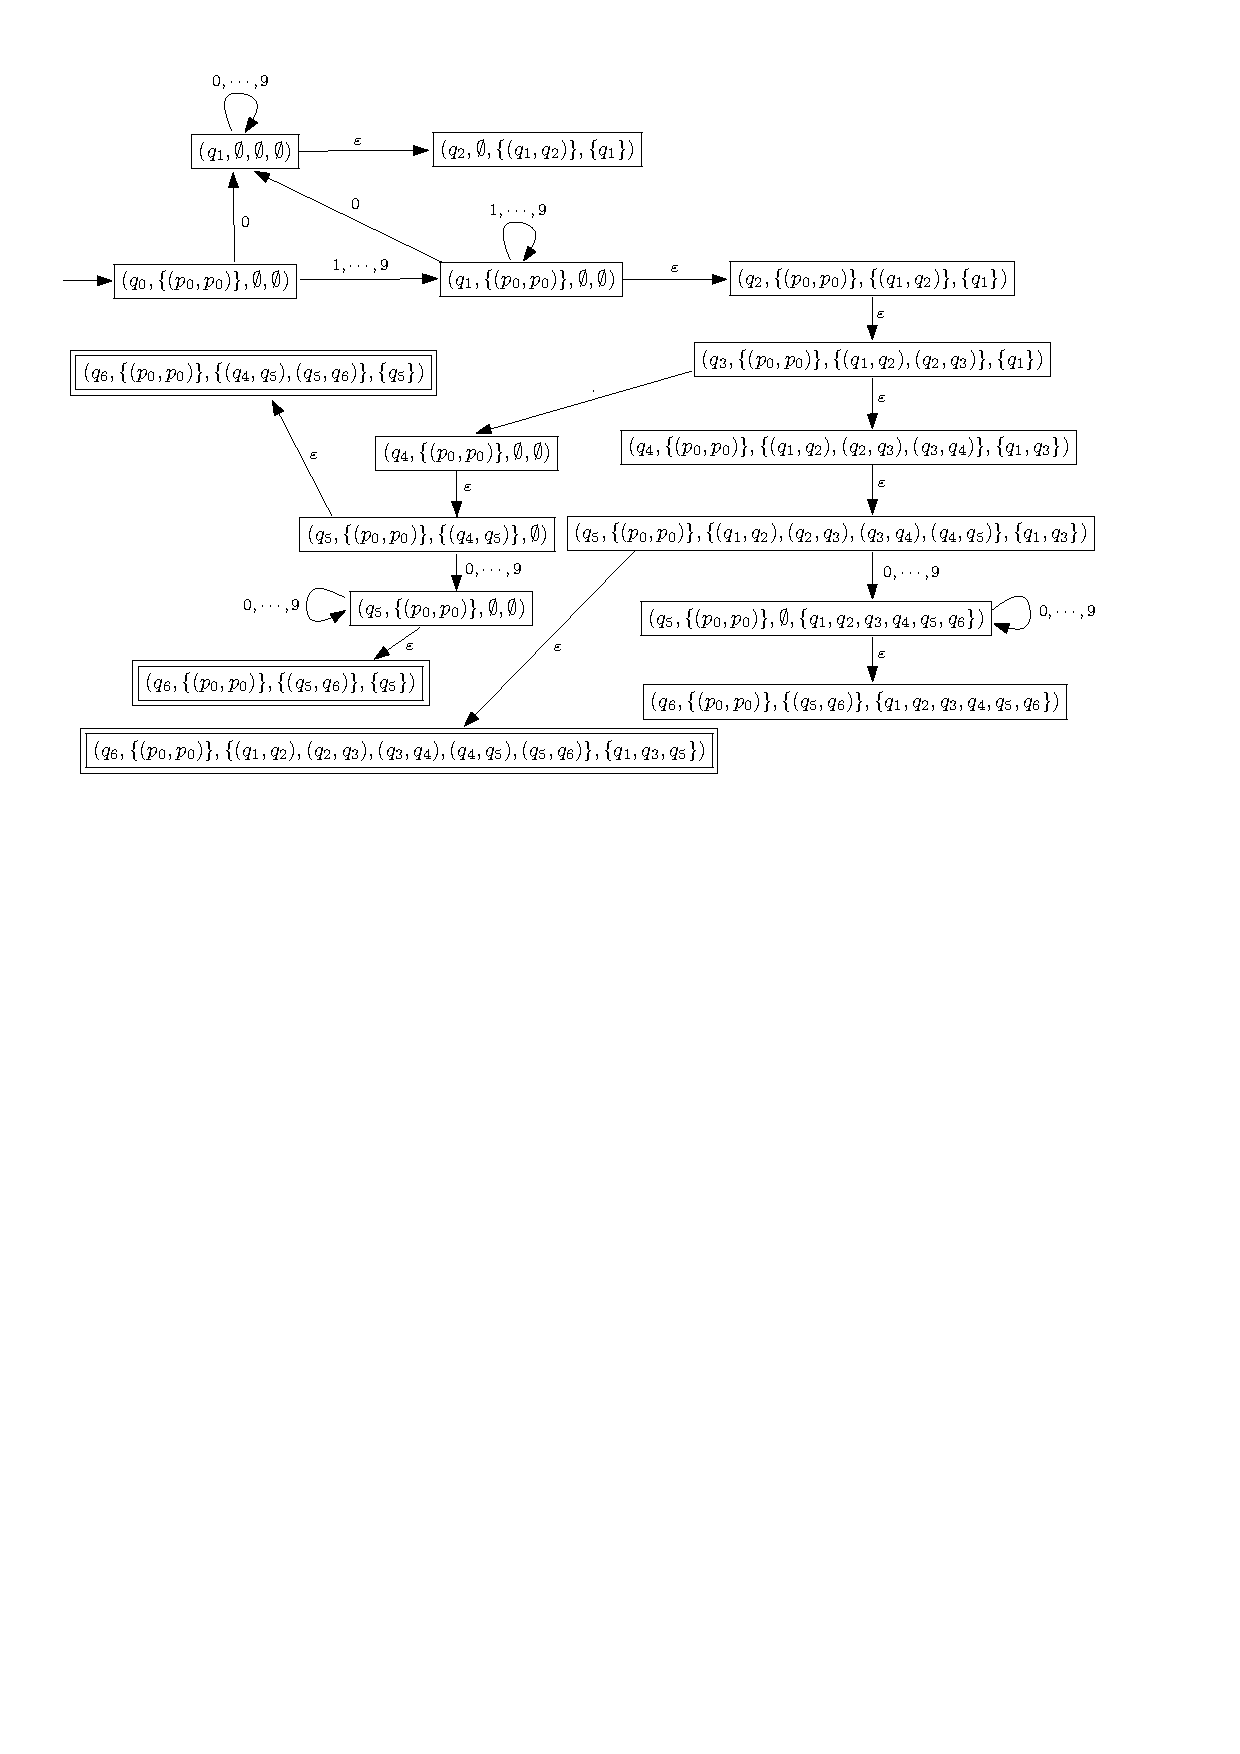
\includegraphics[width = \textwidth]{psst-preimage-example-new.pdf}
\caption{The FA defining $\cR^{-1}_{\cT_{\tt match_{decimalReg,1}}}(\Lang(\Aut))$}
\label{fig-psst-preimage-exmp}
\end{figure}

%%%%%%%%%%%%%%%%%%%%%%%%%%%%%%%%%%%
%%%%%%%%%%%%%%%%%%%%%%%%%%%%%%%%%%%
\hide{
\begin{table}[t]
\centering
\caption{the actual $\cB$ state in Figure 
\label{table:psst-preimage}
\ref{fig-psst-preimage-exmp}}
\begin{tabular}{|c|c|}
    \hline
    Symbol & State of $\cB$\\
    \hline
    $r_0$ & $(q_0, \rho_1, \emptyset, \emptyset)$\\
    \hline
    $r_1$ & $(q_1, \rho_1, \{ (q_0, q_1) \}, \emptyset)$\\
    \hline
    $r_2$ & $(q_2, \rho_1, \{ (q_0, q_1), (q_1, q_2) \}, \{ q_0 \})$\\
    \hline
    $r_3$ & $(q_2, \rho_2, \emptyset, \{ q_0, q_1, q_2 \})$\\
    \hline
    $r_4$ & $(q_2, \rho_1, \emptyset, \{ q_0, q_1, q_2 \})$\\
    \hline
    $r_5$ & $(q_0, \rho_1, \{ (q_0, q_1) (q_1, q_0) \}, \emptyset)$\\
    \hline
    $r_6$ & $(q_0, \rho_2, \emptyset, \emptyset)$\\
    \hline
    $r_7$ & $(q_0, \rho_2, \emptyset, \{ q_0, q_1, q_2 \})$\\
    \hline
    $r_8$ & $(q_1, \rho_2, \{ (q_0, q_1) \}, \{ q_0, q_1, q_2 \})$\\
    \hline
    $r_9$ & $(q_0, \rho_2, \{ (q_0, q_1) (q_1, q_0) \}, \{ q_0, q_1, q_2 \})$\\
    \hline
    $r_{10}$ & $(q_2, \rho_2, \{ (q_0, q_1) (q_1, q_2) \}, \{ q_0, q_1, q_2 \})$\\
    \hline
    $r_{11}$ & $(q_0, \rho_1, \emptyset, \{ q_0, q_1, q_2 \})$\\
    \hline
    $r_{12}$ & $(q_1, \rho_1, \{ (q_0, q_1) \}, \{ q_0, q_1, q_2 \})$\\
    \hline
    $r_{13}$ & $(q_0, \rho_1, \{ (q_0, q_1) (q_1, q_0) \}, \{ q_0, q_1, q_2 \})$\\
    \hline
    $r_{14}$ & $(q_2, \rho_1, \{ (q_0, q_1) (q_1, q_2) \}, \{ q_0, q_1, q_2 \})$\\
    \hline
    $r_{15}$ & $(q_2, \rho_2, \{ (q_0, q_1) (q_1, q_2) \}, \{ q_0 \})$\\
    \hline
    $r_{16}$ & $(q_1, \rho_2, \emptyset, \{ q_0, q_1, q_2 \})$\\
    \hline
    $r_{17}$ & $(q_2, \rho_2, \{ (q_1, q_2) \}, \{ q_0, q_1, q_2 \})$\\
    \hline
    $r_{18}$ & $(q_0, \rho_2, \{ (q_1, q_0) \}, \{ q_0, q_1, q_2 \})$\\
    \hline
    $r_{19}$ & $(q_1, \rho_2, \{ (q_1, q_0) (q_0, q_1) \}, \{ q_0, q_1, q_2 \})$\\
    \hline
    $r_{20}$ & $(q_2, \rho_2, \{ (q_1, q_0) (q_0, q_1) (q_1, q_2) \}, \{ q_0, q_1, q_2 \})$\\
    \hline
    $r_{21}$ & $(q_1, \rho_2, \{ (q_0, q_1) \}, \emptyset)$\\
    \hline
    $r_{22}$ & $(q_0, \rho_2, \{ (q_0, q_1) (q_1, q_0) \}, \emptyset)$\\
    \hline
\end{tabular}
\end{table}
}
%%%%%%%%%%%%%%%%%%%%%%%%%%%%%%%%%%%
%%%%%%%%%%%%%%%%%%%%%%%%%%%%%%%%%%%


\zhilin{stopped here}
\zhilei{changed a little bit}

\subsection{Complexity}

\begin{proposition}[POPL'19]
	The path feasibility problem of the following two fragments is non-elementary: SL with 2FTs, and SL with FTs+replaceAll.
	
	SL[conc, replaceAll, reverse, FFT] is expspace-complete (note that 2FTs in SL are restricted to be one-way and functional)
\end{proposition}

%The same proof strategy can be used for FTs+replaceAll. The 2FTs used in the proof above
%proceed by running completely over the word and producing some output, then silently moving
%back to the beginning of the word. An arbitrary number of passes are made in this way. We
%can simulate this behaviour using FTs and replaceAll.


The main open question is the complexity of the SL fragment with replaceall function and prioritized streaming transducers. Note that PSST can simulate 2FT (adapting Matt's proof?), so we could obtain nonelementary lower bound for SL with PSST.

However, this variant of replaceall is quite different from the replaceall we had before ...

\begin{enumerate}
\item  does  copyless help?
\item how about SL with only this version of replaceall?
\end{enumerate}
